\section{Statistical Learning Theory and Support Vector Machines}
Statistical learning theory deals mainly with \textbf{supervised learning} problems, such that, given:
\begin{itemize}
	\item an input (feature) space: $\mathcal{X}$
	\item an output (label) space: $\mathcal{Y}$ (typically $\mathcal{Y} = \{-1,+1\}$)
\end{itemize}
The question of learning amounts to estimating a functional relationship between the input and the output spaces:
$$f: \mathcal{X} \rightarrow \mathcal{Y}$$
such mapping $f$ is called a \textbf{classifier}. In order to do this, we have access to some (labeled) training data:
$$(x_1,y_1), \dots, (x_n, y_n) \in \mathcal{X} \times \mathcal{Y}$$
A classification algorithm is a procedure that takes the training data as input and outputs a classifier $f$.\\
In statistical learning theory, the following \textbf{assumptions} are made:
\begin{itemize}
	\item There exists a joint probability distribution $P$ on $\mathcal{X} \times \mathcal{Y}$. The $P$ distribution is unknown at the time of learning. 
	\item The training examples $(x_i, y_i)$ are sampled independently from $P$ (iid sampling).
\end{itemize}
Moreover:
\begin{itemize}
	\item No assumption on the unknown distribution $P$.
	\item $P$ is fixed.
	\item Non-deterministic labels due to label noise or overlapping.
\end{itemize}
What is needed is also a measure of "how good" a function $f$ is when used as a classifier. A \textbf{loss function} measures the "cost" of classifying instance $x \in \mathcal{X}$ as $y \in \mathcal{Y}$. In other words, a loss function measures the cost of classification and miss-classification of an element. The simplest loss function in classification problems is the $0-1$ loss (or miss-classification error):
$$
\ell ( X , Y , f ( X ) ) = 
\left\{ \begin{array} { l l } { 1 } & { \text { if } f ( X ) \neq Y } \\ 
{ 0 } & { \text { otherwise } } \end{array} \right.
$$
The \textbf{risk} of a function is the average loss over data points generated according to the underlying distribution $P$:
$$R ( f ) = E ( \ell ( X , Y , f ( X ) ) )$$
The best classifier is the one with the smallest risk $R(f)$, since it gives us a measure of goodness of the classifier.
$$R(f) = \sum_{x \in X}p(x)\ell(x,y,f(x))$$
This theoretical result cannot be computed in real experiments since the underlying distribution is unknown, and estimating it can be very expensive in a high dimensional space.\\
Among all possible classifiers, the best one is the \textbf{Bayes classifier}:
$$
f _ { \text {Bayes} } ( x ) = \left\{ \begin{array} { l l } { 1 } & { \text { if } P ( Y = 1 | X = x ) \geq 0.5 } \\ { - 1 } & { \text { otherwise } } \end{array} \right.
$$
In practice, it is impossible to directly compute the Bayes classifier as the underlying probability distribution $P$ is unknown to the learner, the idea of estimating $P$ from data doesn't usually work.

\paragraph{Bayes' Theorem.} The Bayes' theorem is defined by the following formula:
$$
P ( h | e ) = \frac { P ( e | h ) P ( h ) } { P ( e ) } = \frac { P ( e | h ) P ( h ) } { P ( e | h ) P ( h ) + P ( e | \neg h ) P ( \neg h ) }
$$
where:
\begin{itemize}
	\item $P(h)$: prior probability of hypothesis $h$.
	\item $P(h|e)$: posterior probability of hypothesis $h$ (in the light of evidence $e$).
	\item $P(e|h)$: "likelihood" of evidence $e$ on hypothesis $h$.
\end{itemize}

\subsection{The classification problem} 
Given:
\begin{itemize}
	\item A set of training points $(x_1,y_1), \dots, (x_n, y_n) \in \mathcal{X} \times \mathcal{Y}$ drawn iid from an unknown distribution $P$.
	\item A loss function.
\end{itemize}
Determine a function $f:\mathcal{X} \rightarrow \mathcal{Y}$ which has risk $R(f)$ as close as possible to the risk of the Bayes classifier. Since we don't known the distribution of $P$ it is impossible to compute the Bayes error and the risk of a function $f$.

\paragraph{NN Classifier} It is a non-parametric method used for classification. Given a new point to be classified $x$, the NN classifier search in the training set for the closest point $z$ to $x$ and assign the same label of $z$ to $x$. Positions in the space of the training points define a partition of the input space (decision regions). The resulting partition follows the property of the \textbf{Voronoi Tessellation}. The assumption made by the NN classifier is that the training set is fixed, no updates are done during test, otherwise it is necessary to re-train it. \\
An extension of this classifier is called \textbf{KNN} which, instead  of considering only the closest point, it considers the k-closest points to $x$ and assigns the class with the greater number of voting. This is done in order to improve the robustness of the classifier.\\
In summary we have the following variations of NN:
\begin{itemize}
	\item $k$-NN rule: use the $k$ nearest neighbors and take a majority vote.
	\item $k_n$-NN rule: the same as above, for $k_n$ growing with $n$.
\end{itemize}
With the NN classifier basically we don't have learning and so we have two fundamental problems:
\begin{itemize}
	\item \textbf{Search problem}, require an efficient algorithm to find the closest points.
	\item \textbf{Storage}, in order to work with the entire training set it must be loaded in memory.
\end{itemize}

\paragraph{Estimate P}
One of the assumptions that we said at the beginning is that the probability distribution $P$ is unknown, but we can think to estimate it. A good estimator is:
$$P(x) = \frac{\frac{K}{n}}{V}$$
where $V$ is the volume and $K$  is the number of observations in $V$. We know that each observation has probability $\frac{1}{nv}$. From this we can think that when $n \rightarrow \infty$ and $K(n) \rightarrow \infty$ the estimate density is equal to the real density, of course it can be computationally expensive in very high dimensional space.

\subsection{How good is the NN rule?.} Cover and Thomas showed that:
$$R(f_{bayes}) \leq R_\infty \leq 2R(f_{Bayes})$$
where $R_{\infty}$ denotes the expected error rate of NN when the sample size tends to infinity. Remember that $R(f_{bayes})$ is the lower bound since we said that the Bayes classifier is the best one. We cannot say anything stronger as there are probability distributions for which the performance of the NN rule achieves either the upper or lower bound. 
\begin{thm}[Stone Theorem (1977)]
	If $n \rightarrow \infty$ and $k \rightarrow \infty$, such that $k/n \rightarrow 0$, then for all probability distributions $R(k_n\text{-NN}) \rightarrow R(f_{Bayes})$ (that is, the $k_n$-NN rule is "universally Bayes consistent")
\end{thm}

\paragraph*{The Empirical Risk Minimization principle.} Instead of looking for a function which minimizes the true risk $R(f)$, we try to find one which minimizes the \textbf{empirical risk}:
$$R _ { \mathrm { emp } } ( f ) = \frac { 1 } { n } \sum _ { i = 1 } ^ { n } \ell \left( X _ { i } , Y _ { i } , f \left( X _ { i } \right) \right)$$
Given training data $(x_1,y_1), \dots, (x_n, y_n) \in \mathcal{X} \times \mathcal{Y}$, a function space $\mathcal{F}$, and a loss function, we define the classifier $f_n$ as:
$$f _ { n } = \underset { f \in \mathcal { F } } { \operatorname { argmin } } \operatorname { R } _ { \mathrm { emp } } ( f )$$
This approach is called the \textbf{empirical risk minimization} (ERM) induction principle, the motivation of which comes from the law of large numbers.
\subsection{Estimation vs approximation}
Ideally we want to make $R(f_n) - R(f_{Bayes})$ as small as possible, as $n \rightarrow \infty$. Denoting by $f_{\mathcal{ F }}$ the best classifier in $\mathcal{ F }$, the difference can be decomposed as:
$$R \left( f _ { n } \right) - R \left( f _ { B a y e s } \right) = \underbrace{\left( R \left( f _ { n } \right) - R \left( f _ { \mathcal { F } } \right) \right)}_{\text{estimation error}} + \underbrace{\left( R \left( f _ { \mathcal { F } } \right) - R \left( f _ { \text {Bayes} } \right) \right)}_{\text{approximation error}}$$

\begin{itemize}
	\item $R(f_n)$ is the risk of my classifier.
	\item $R(f_\mathcal{ F })$ is the risk of the best classifier $f$ on the family $\mathcal{ F }$.
	\item $R \left( f _ { \text {Bayes} } \right)$ is the risk of the best classifier.
\end{itemize}
\image{img/estimation}{Estimation vs approximation.}{0.35}
According to the complexity of $\mathcal{ F }$ we can have:
\begin{itemize}
	\item small complexity of $\mathcal{ F }$: small estimation error, large approximation error (\textit{underfitting})
	\item large complexity of $\mathcal{ F }$: large estimation error, small approximation error (\textit{overfitting})
\end{itemize}
The best overall risk is achieved for "moderate" complexity.
\image{img/overunderfitting}{Underfitting vs Overfitting graph}{0.55}
\image{img/modelselection}{Model selection.}{0.8}

\paragraph*{Shattering.} A set of $n$ instances $x_1, \dots, x_n$ from the input space $\mathcal{X}$ is said to be \textit{shattered} by a function class $\mathcal{ F }$ if all the $2^n$ labelings of them can be generated using functions from $\mathcal{ F }$.\\ 
For instance, with $\mathcal{ F }$ as a linear decision functions (straight lines) in the plane, we can have:
\begin{enumerate}[label=(\alph*)]
	\item Any set of 3 non-collinear points shatters $\mathcal{ F }$
	\item No set of 4 points can shatter $\mathcal{ F }$
\end{enumerate}
\imageb{img/shattered}{0.85}

\paragraph*{The VC dimension.} The \textbf{VC dimension} of a function class $\mathcal{ F }$, denoted $VC(\mathcal{ F })$, is the largest integer $h$ such that there exists a sample of size $h$ which is shattered by $\mathcal{ F }$. It is a measure of complexity of a function class.\\
If arbitrarily large samples can be shattered, then $VC(\mathcal{ F }) = \infty$.\\
For example:
\begin{itemize}
	\item $\mathcal{ F }$ = linear decision functions in $\mathbb{R}^2 \rightarrow VC(\mathcal{ F }) = 3$
	\item $\mathcal{ F }$ = linear decision functions (hyperplanes) in $\mathbb{R}^n \rightarrow VC(\mathcal{ F }) = n+1$ 
	\item $\mathcal{ F }$ = multi-layer perceptrons with $W$ weights $\rightarrow VC(\mathcal{ F }) = O(W~\log( W))$
	\item $\mathcal{ F }$ = nearest neighbor classifiers $\rightarrow VC(\mathcal{ F }) = \infty$
\end{itemize}


The VC dimension for the classifier depends on the dimension of space that your data points belong to. In your problem, if your mean $x\in \mathbb{R}^2$, then the VC dimension is $3$. For $\mathbb{R}^2$, you can always shatter any three general position points ("general position" means they do not coincidentally lie on the same line). For instance, consider three points $(0,0)$, $(0,1)$, $(1,0)$. No matter how you assign labels to them, you can always separate them by a line. If you consider three points $(0,0)$, $(0,1)$, $(1,0)$, $(1,1)$ with label $[+,-,-,+]$, this is the "xor" case which cannot be separated by a line. For $x\in\mathbb{R}$, then the VC dimension is 2 because you cannot separate $+-+$. In general for $x\in\mathbb{R}^d$, the VC dimension for a linear classifier is $d+1$.\\

The VC dimension is in general not related to the number of free parameters of a model.\\
For all $f \in \mathcal{ F }$, with probability at least $1-\delta$, we have:
$$
R ( f ) \leq R _ { \mathrm { emp } } ( f ) + \underbrace{\sqrt { \frac { h ( \log ( 2 n / h ) + 1 ) - \log ( \delta / 4 ) } { n } }}_{\text{VC confidence}}
$$
where $h=VC(\mathcal{ F })$ is the VC dimension of the family $F$, $\delta$ is a tolerant parameter, and $n$ is the sample size. We can read this results as:\\

\textit{With probability approaching  1, no matter what the unknown probability distribution, given more and more data, the expected error for the functions that ERM endorses at each stage eventually approaches the minimum value of expected error of the functions in $\mathcal{ F }$ if and only if $\mathcal{ F }$ has finite VC dimension. If VC dimension is equal to $\infty$, like in the KNN case, we have that $R_\text{emp}(f) = 0$ and so $R(f) \leq \infty$ which is meaningless.}\\

Another key of reading is that since the second term $R_\text{emp}\dots$ is an upper bound, if it is small so also $R(f)$ will be. This result is fundamental due to the fact that we have no knowledge about $P$ and so we cannot compute $R(f)$, but we can have a bound for it using the second quantity. Indirectly we want to reduce the bound so that at the end the resulting risk is minimized.

\paragraph*{Structural Risk minimization.} It is a general framework for choosing the best classifier. Empirical Risk Minimization takes only care of the \textit{estimation} error (variance) but it is not concerned with the \textbf{approximation error} (bias). The optimal model is found by striking a balance between the empirical risk and the capacity of the function class $\mathcal{ F }$ (ex: the VC dimension).\\
The basic idea of \textit{Structural Risk Minimization} (SRM) is:
\begin{enumerate}
	\item Construct a nested structure for family of function classes $\mathcal{ F }_1 \subset \mathcal{ F }_2 \subset \dots$ with non-decreasing VC dimension $(VC(\mathcal{ F }_1) \leq VC(\mathcal{ F }_2) \leq \dots)$
	\item For each class $\mathcal{ F }_i$, find the solution $f_i$ that minimizes the empirical risk.
	\item Choose the function class $\mathcal{ F }_i$, and the corresponding solution $f_i$ that minimizes the risk bound (= empirical risk + VC confidence) 
\end{enumerate}

\image{img/risk_minimization}{Structural risk minimization.}{0.55}
\newpage
\subsection{Support Vector Machine}
In this section we are going to deal with a very well known supervised learning algorithm, called \textbf{Support Vector Machine}. We will see that it can be written as an intuitive optimization problem and can be easily extended to work very well with non-linear patterns or in high dimensional spaces.\\

SVM belongs to the class of discriminative classifiers since its goal consists on learning the class boundary between the two classes $y$ starting from features $x$. From now, we'll use $y\in\{-1,1\}$ to denote the class labels.
We can formally define the SVM linear classifier in this way:
$$h_{w,b}(x) = g(w^Tx + b)$$
$$
g(z)=
\begin{cases}
1\qquad \text{if} \quad z \geq 0\\
-1\qquad \text{otherwise}\\
\end{cases}
$$
Where $w^T + b$ represents a \textbf{separating hyperplane} for the two classes, and $g(z)$ is the decision function which returns the predicted class for the observation $x$.
In our problem the classifier would then predict $1$ if $h_{w,b}(x) \geq 0$, which is equivalent of considering $w^Tx + b \geq 0$, and $-1$ otherwise.
We define the probability of classification given an observation $x$ as:
$$p(y = 1 | x; w,b)$$
This quantity over here represent the confidence of our classifier on assigning the label $1$ to the input value $x$. We can also say that the larger $w^Tx + b$ is, the higher is the confidence that the label is $1$. Remember that the function $g$ is our decision function, so if we are strongly distant from the $0$ we have high confidence of the class $1$, otherwise if we are close to the $0$ the function $g$ assigns the label $1$ but now the confidence is lower. In other words this probability represent the confidence about the algorithm classification.\\
This result is a consequence of the fact that if $w^Tx + b$ increase then also $h_{w,b}(x)= p(y = 1 | x; w,b)$ becomes larger. The same thing is valid with label $-1$, in this case we would like to have $w^Tx + b$ as small as possible $w^Tx + b \ll 0$.\\

\begin{figure}[!h]
	\begin{minipage}[t]{0.5\linewidth}
		\centering
		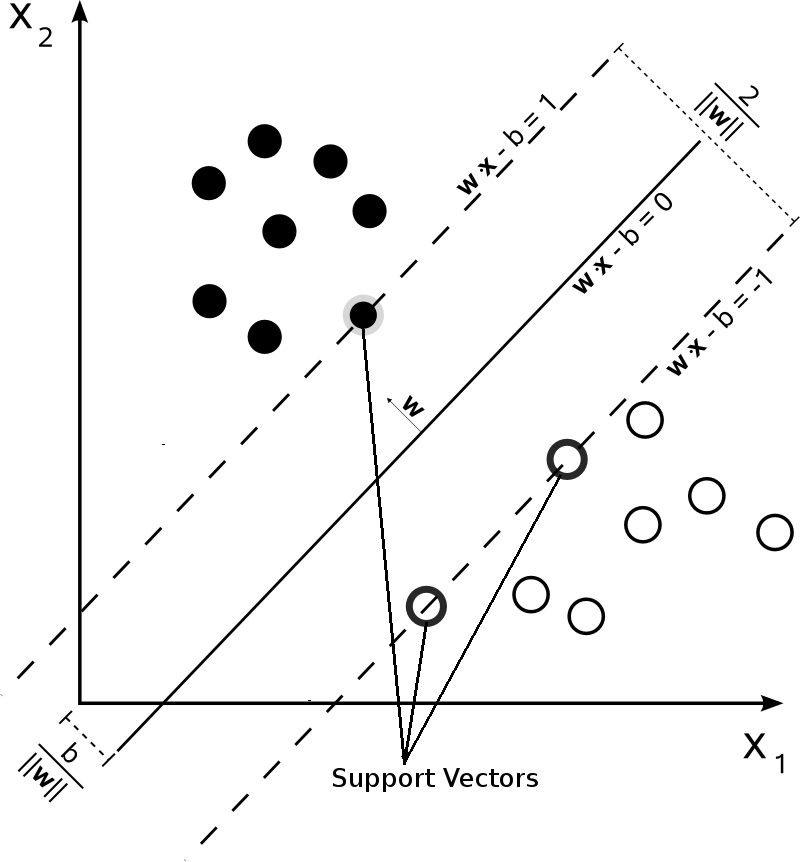
\includegraphics[width=0.8\textwidth]{img/SVMPlot2.png}
		\caption{Support Vector Machines classifier}
		\label{svmclassifier}
	\end{minipage}
	\hspace{0.1cm}
	\begin{minipage}[t]{0.5\linewidth} 
		\centering
		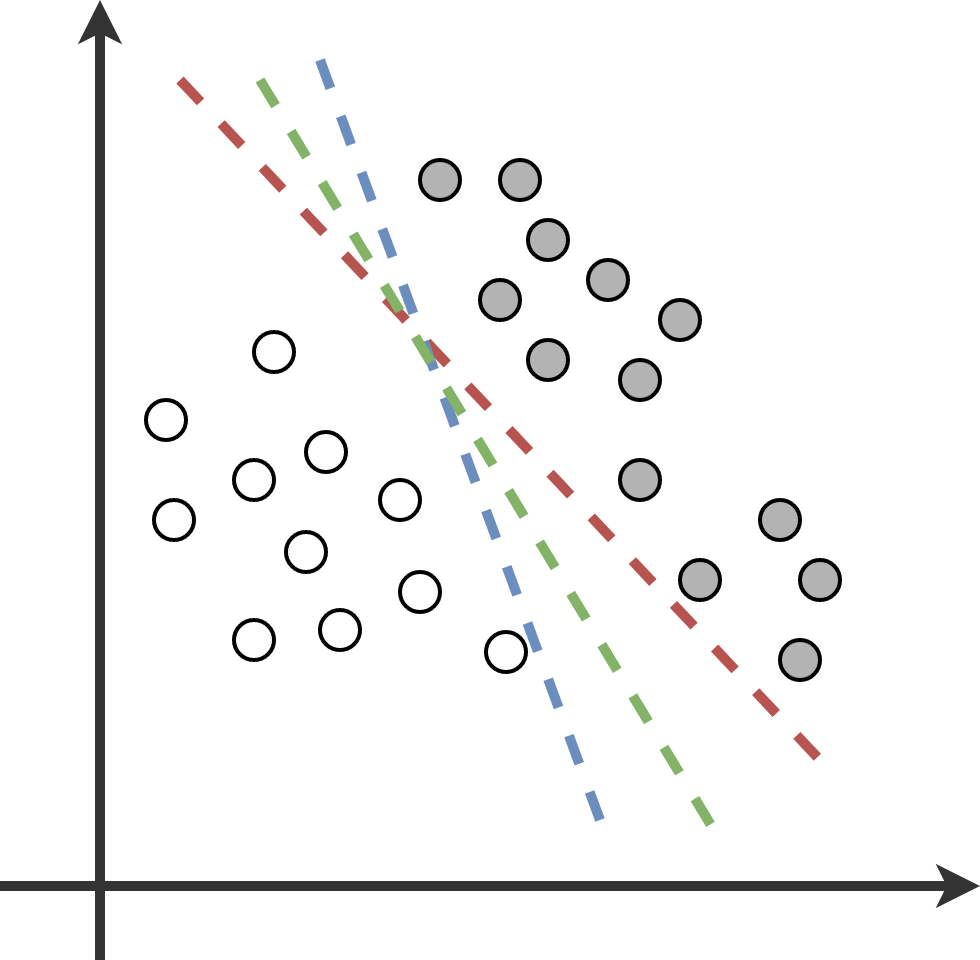
\includegraphics[width=0.9\textwidth]{img/separating-lines.png}
		\caption{Possible separating hyperplanes}
		\label{svmmargindecison}
	\end{minipage}        
\end{figure} 

Figure \ref{svmclassifier} shows an application of a SVM classifier. In this example we have two classes $1$ and $-1$ represented in a $2$ dimensional space using respectively filled points and empty ones. The line given by the equation $w^Tx + b = 0$ defines the \textbf{separate hyperplane} which works as a \textbf{decision boundary} of our problem. Points that below the plane are labeled with $y = -1$, since $w^Tx+b < 0$, otherwise they are labeled with $y = 1$.\\

Considering Figure \ref{svmmargindecison} we can notice that we can define different separating hyperplanes, and all of them provides $100\%$ of accuracy on this training set. This concept introduces a problem which must be considered: \textit{Which is the right hyperplane?} In general it is possible to find an infinite number of hyperplanes that separate the two classes, but they can produce different results/performance and also they can have effects on the robustness of the classifier.\\
Before going in details of the best hyperplane it is necessary to introduce the following concepts: \textbf{functional margin} and \textbf{geometric margin}.

\paragraph{Functional margin} It is a testing function that verifies if a particular point is properly classified or not.
$$\hat{\gamma}^{(i)} = y^{(i)}(w^Tx^{(i)} + b)$$
When $\hat{\gamma}^{(i)} > 0$ the prediction of the observation $i$ is correct, and the larger is the functional margin result the greater is the confidence of the current prediction. However it cannot be considered as a very good measure of confidence since it is affected by the length of the two vectors $w, b$. In fact, considering the pair $(\alpha w, \alpha b)$ we can notice that the new functional margin is multiplied by the factor $\alpha$. For that reason could be reasonable to set $||w||_2 = 1$, but we will discuss about it later.


\paragraph{Geometric margin} It represents the euclidean distance between a point and the decision boundary.
\image{img/geometricMargin.png}{Geometric margin}{0.45}
Considering the previous figure, $A$ is a point representing the $i^{th}$ observation and $B$ is a point on the straight line defined by $w^TB+b = 0$. We can so define the geometrical margin $\gamma^{(i)}$ as the length of the segment $AB$. \\

Now that we have defined the notion of geometric and functional margin it is possible to give an idea of which is the best hyperplane. This concept, as we are going to see, is strictly related to the two margins. We define the \textbf{geometric margin} $\gamma$ and the \textbf{functional margin} $\hat{\gamma}$ respect to the training set $S = \{(x^{(i)},y^{(i)}); i = 1,\dots,m \}$ the following value:
$$\gamma = \underset{i = 1,\dots,m}{\text{min }}\gamma^{(i)}$$
$$\hat{\gamma} = \underset{i = 1,\dots,m}{\text{min }}\hat{\gamma}^{(i)}$$


This values $\gamma$ represents the distance from the decision boundary to the closest point, and it is also called \textbf{margin}. Distance to the closest training point is called the margin. An interesting property of the geometric margin is that it is related with the functional margin by the following definition: $\gamma = \frac{\hat{\gamma}}{||w||}$. \\
The idea of an SVM classifier is to find a separating hyperplane which \textbf{maximizes the geometric margin}. The resulting hyperplane is so considered as the best one since it separates better then other ones the two classes. Intuitively, the farthest is the boundary from the points, the greater is the confidence.\\
Formally speaking the main goal of Support Vector Machine is to solve the following optimization problem:

\begin{equation*}
\begin{aligned}
&\text{max }_{\gamma,w,b} \quad \gamma\\
&\text{s.t.} \quad y^{(i)}(w^Tx^{(i)}+b) \geq \gamma \qquad i = 1,\dots, m\\
&||w|| = 1
\end{aligned}
\end{equation*}
where $y^{(i)}(w^Tx^{(i)}+b) \geq \gamma$ means that points must have minimum distance $\gamma$ from the decision boundary.
The constraint $||w|| = 1$, that we have seen previously, is now introduced to enforce that the functional margin is equal to the geometric one, so that the problem can be rewritten as:
\begin{equation*}
\begin{aligned}
&\text{max }_{\hat{\gamma},w,b} \quad \frac{\hat{\gamma}}{||w||}\\
&\text{s.t.} \quad y^{(i)}(w^Tx^{(i)}+b) \geq \hat{\gamma} \qquad i = 1,\dots, m\\
\end{aligned}
\end{equation*}

Now the non-convex constraint $||w|| = 1$ is introduced directly inside the target function and instead of considering the geometric margin the optimization problem is re-formulated in terms of functional margin. Now imposing the scaling constraint $\hat{\gamma}$ = 1 it is possible to rewrite the same optimization problem as a minimization of $||w||^2$:
\begin{equation}\label{svmopt}
\begin{aligned}
&\text{min }_{\gamma,w,b} \quad \frac{1}{2}||w||^2\\
&\text{s.t.} \quad y^{(i)}(w^Tx^{(i)}+b) \geq 1 \qquad i = 1,\dots, m\\
\end{aligned}
\end{equation}
This formulation represent an optimization problem on a convex function and with only linear constraints. Due to the nature of the problem we have a unique minimum solution which represents \textbf{optimal margin classifier}. An interesting thing of SVM is that it does not require to check for all the points, but it considers  only the support vectors. They are showed in Figure \ref{svmclassifier} and they represents the points with distance equal to the minimum margin from the decision boundary. SVM is only affected by these points, all the other ones can move freely. The advantage of SVM is that instead of considering all the possible points SV from the training set it considers only these points to determine the decision boundary. \\

In order to solve constrained Problem \ref{svmopt} we introduce the concept of Lagrange multipliers. Using the \textbf{Lagrange} function with $N$ Lagrange multipliers $\Lambda = (\lambda_1,\dots,\lambda_N)$ it is possible to rewrite the correspondent optimization problem, with parameters $w$ and $b$, into an identical one but with parameters $(\lambda_1,\dots,\lambda_N)$. Taking advantage of the dual representation, that allows to convert an original min/max problem into another one which is equivalent but with max/min formulation, we can write the new optimization problem as follow:

\begin{equation}
\quad L(w,b,\Lambda) = \frac{1}{2}||w||^2 - \underbrace{\sum_{i = 1}^{N}\lambda_i[y_i(w^Tx_i+b)-1]}_{\text{Sum of constraints}}\\
\end{equation}
Note that thanks to the dual representation we have converted a constrained problem into an unconstrained one (which is easier to solve). \\

\noindent\fbox{%
	\parbox{\textwidth}{%
\paragraph{Convert constrained P into an unconstrained one}  
Given the following constrained optimization problem:
\begin{equation}\label{constraint}
\begin{aligned}
& \min ~ f(x)\\
&\text{s.t.}~ x \in \mathcal{D}\\
\end{aligned}
\end{equation}
\image{img/constrainedSpace.png}{Constrained space for the Optimization Problem \ref{constraint}.}{0.3}
The unconstrained version can be defined:
\begin{equation}\label{unconstraint}
\begin{aligned}
& \min ~ f(x)\\
&\text{s.t.}~ x \in \mathbb{R}^n	\\
\end{aligned}
\end{equation}
Of course the solutions of problems \ref{constraint} and \ref{unconstraint} can be different. For that reason we can introduce a new formulation that tries to produce the same results:
\begin{equation}\label{penaltyconstraint}
\begin{aligned}
& \min ~ f(x) + \lambda p(x)\\
&\text{s.t.}~ x \in \mathbb{R}^n	\\
\end{aligned}
\end{equation}
where $p(x)$ is a penalty function equal to $0$ if $x\in \mathcal{D}$, otherwise it is greater than $0$. The greater is the distance from $\mathcal{D}$ the greater is the penalty. The advantage of this formulation is that now we have an unconstrained problem. The same idea is adopted by the dual representation with Lagrangian Multipliers.\\
    }%
}
\newline

The goal is to find a function parameterized only by Lagrangian Multipliers. Setting the derivatives of $L(w,b,\Lambda)$ to zero:
$$\frac{\partial L(w,b,\Lambda)}{\partial w} = w- \sum_{i = 1}^{N}\lambda_iy_ix_i = 0 \qquad \implies \qquad w = \sum_{i = 1}^{N}\lambda_iy_ix_i$$
$$
\frac{\partial L(w,b,\Lambda)}{\partial b} =\sum_{i = 1}^{N}\lambda_iy_i = 0 
$$
We obtain a new formulation of the optimization problem expressed with only lagrangian multipliers:

\begin{equation*}
\begin{aligned}
&\text{max }\quad L_D(\lambda_1,\dots,\lambda_m) = \sum_{i = 1}^{m}\lambda_i - \frac{1}{2}\sum_{i = 1}^{m}\sum_{j = 1}^{m}\lambda_i\lambda_jy_iy_jx_i^Tx_j\\
&\text{s.t.} \quad \sum_{i = 1}^{m}\lambda_iy_i= 0 \qquad \lambda_i \geq 0, \forall i = 1,\dots,m\\
\end{aligned}
\end{equation*}
Note that the training vectors appears only as \textit{dot products}, and the advantage of using this formulation is that only support vectors will have Lagrange multipliers such that $\lambda_i > 0$ and the others will be essentially equal to zero (sparse solution). The SVM complexity is given only by the support vectors. Now the maximum margin hyperplane is given by:
$$\sum_{i = 1}^{m} y_i \lambda_ix_i^Tx+b = 0$$

If $\Lambda = (\lambda_1,\dots, \lambda_N)$ is the solution of the dual optimization problem, then:
\begin{itemize}
	\item The weight vector of the maximum margin hyperplane is:
	$w = \sum_{i = 1}^{N} y_i\lambda_ix_i$
	\item The corresponding discriminant function (separating hyperplane) is:
	$$f(x) = w^Tx+b =  \sum_{i = 1}^{N} y_i\lambda_ix_i^Tx_i + b$$
	\item The linear SVM classifier $g: \mathbb{R}^n \rightarrow \{-1,1\}$ is:
	$$g(x) = \text{sign}(w^Tx+b =  \sum_{i = 1}^{N} y_i\lambda_ix_i^Tx_i + b)$$
\end{itemize}
For support vector we have:
$$y_i(\sum_{i = 1}^{N} y_i\lambda_ix_i^Tx_i + b) = \gamma$$
For simplicity we consider $\gamma = 1$. Since SVM is affected only by support vectors we can derive:
$$b = \frac{1}{|SV|}\sum_{i\in SV}\Large(y_i-\sum_{j=1}^{N}y_j\lambda_jx_j^Tx_i\Large)$$
where SV is the set of support vectors.

\subsubsection{SVM error function}
The generic loss function adopted for training a support vector machine is the \textbf{Hinge loss function}. 
$$L_{\text{hinge}} = \max \{0, 1- y_if(x_i)\}$$
\image{img/hingeloss.png}{Hinge loss function.}{0.45}
$$E = \sum\limits_{i=1}^N\max\{0,1-y_if(x_i)\}+\frac{1}{2}\sum\limits_{j = 1}^dw_j^2$$

\begin{itemize}
	\item $\sum\limits_{i=1}^N\max\{0,1-y_if(x_i)\}$, hinge loss function over all data points.
	\item $\frac{1}{2}\sum\limits_{j = 1}^dw_j^2$, proportional to the inverse of the margin.
\end{itemize}
Notice that the hinge loss function is not differentiable on $1$, we can't apply the gradient descent procedure. The solution of this problem consists on using \textbf{quadratic programming (QP)} algorithms, since $E$ is a quadratic function with linear constraints.


\subsubsection{SVM's and the VC dimension}
\paragraph{Theorem (Vapnik)} Consider hyperplanes $w^Tx+b= 0$ in canonical form, that is such that:
$$\min\limits_{1\leq i \leq N}|w^Tx_i+b| = \gamma = 1$$
Then the set of decision functions $g(x) = sgn(w^Tx+b = 0)$ that satisfy the constraint $||w|| < \gamma$ has a VC dimension $h$ satisfying:
$$h \leq R^2\gamma^2$$
where $R$ is the smallest radius of the sphere around the origin containing all the training points. Note that dropping the condition $||w|| < \gamma$ leads to a VC dimension equal to $n+1$. Hence, the constraint allows us to work in high-dimension spaces. \\
From the previous theorem and from:
$$R(f) \leq R_{\text{emp}}(f) + \sqrt{\frac{h(\log(\frac{2n}{h})+1)-\log(\frac{\sigma}{4})}{n}}$$
we have:
\begin{itemize}
	\item By maximizing the margin, or equivalent by minimizing $||w||$, we are in fact minimizing the VC dimension of the SVM.
	\item The minimization of the expected risk depends on both minimizing the empirical risk and the confidence interval.
	\item The confidence interval depends mainly on the ratio $\frac{h}{n}$.
	\item SVM algorithm minimizes both the empirical risk and the confidence interval.
	\item SVM directly implements the structural risk minimization principle.
\end{itemize}

\subsubsection{Outliers: soft margins}
One of the problem of SVM is to make decisions in presence of outliers.
\image{img/outlierSVM1.png}{Outliers effects on an SVM.}{0.55}
In the previous image is showed the effect that can have a single outlier. We can make two types of decision: correct classify it reducing the robustness of the classifier, or leave it miss-classified. The strategy which is commonly adopted is the second one, otherwise with the first one we can find decision boundaries that work very well on the training set, but they does not provide optimal performance during testing. In order to reduce the effects of miss-classification we adopt some \textbf{slack variables}, useful for allowing some errors in the boundary.
\image{img/outliersSVM.png}{Outliers effects on an SVM with slack variables.}{0.55}
Now the optimization problem can be re-formulated:
\begin{equation*}
\begin{aligned}
&\text{minimize} \frac{1}{2}||w||^2+ C\sum\limits_{i = 1}^N\xi_i\\
&\text{subject to } y_i(w^Tx_i-b)\geq 1 - \xi_i\\
&\xi_i \geq 0 \qquad i = 1,\dots,N
\end{aligned}
\end{equation*}
The only parameter C controls the tradeoff between the accuracy with respect to the training data and the maximization of the margin. It can be interpreted also as a regularization term:
\begin{itemize}
	\item small $C$ allows constraints to be easily ignored \textit{(large margin)}.
	\item large $C$ makes constraints hard to ignore \textit{(narrow margin)}.
	\item $C = \infty$ enforces all constraints \textit{(hard margin)}.
\end{itemize}
The dual representation of the problem can be reformulated as follows:
\begin{equation*}
\begin{aligned}
&\text{max }\quad L_D(\lambda_1,\dots,\lambda_m) = \sum_{i = 1}^{m}\lambda_i - \frac{1}{2}\sum_{i = 1}^{m}\sum_{j = 1}^{m}\lambda_i\lambda_jy_iy_jx_i^Tx_j\\
&\text{s.t.} \quad \sum_{i = 1}^{m}\lambda_iy_i= 0 \qquad \lambda_i \geq 0, \forall i = 1,\dots,m\\
& 0 \leq \lambda_i \leq C \qquad \forall i = 1,\dots, N
\end{aligned}
\end{equation*}
The hyperplanes whose weights vector solves this quadratic optimization problem are called the \textbf{soft margin hyperplanes}. The soft-margin optimization problem is equivalent to that of the maximum margin hyperplanes with the additional constraint $\lambda_i \leq C$ (box constraints). This approach limits the effect of the outliers (for which $\lambda_i$ tends to be large).

\image{img/hinglosswithslack.png}{Hinge loss function with slack variables.}{0.8}

\image{img/csvm.png}{Effect of C on the decision boundary.}{0.7}

\subsubsection{Kernel Trick}
Until now we worked with the assumption that the space is linearly separable, but SVM allows a strategy called \textbf{kernel trick} for learning a possible separating hyperplane in a new space.
In some cases could be interesting or evaluating not the original space but a transformation of it, for instance when in the original space data points are not linearly separable. We define a function $\phi(x)$ as the function that applies a mapping of a feature vector to another one. The SVM algorithm now instead of considering the vector $x$ learns using the resulting vector of $\phi(x)$. A \textbf{kernel} function is nothing else that an inner product between feature mappings of $\phi$:
$$K(x,z) = \phi(x)^T\phi(z)$$

\paragraph{Cover's Theorem} \textit{A complex pattern-classification problem cast in a high-dimensional space non-linearly is more likely to be linearly separable than in a low-dimension space.}\\

The power of SVM's resides in the fact that they represent a robust and efficient implementation of Cover's theorem.
Informally speaking a kernel function is a similarity measure between the feature mapping $x$ and $z$.
The advantage of using this technique is that it allows to learn in the high dimensional feature space of a transformation of it defining a function $\phi$. 
Since the SVM algorithm works with only inner products between input vectors ($x$,$z$), then we can replace the simple inner product with a kernel function in order to learn in a different feature space that in some cases could be more efficient. But there is a restriction on the function $K$, it must satisfy the following property in order to be considered a \textbf{valid kernel}:
$$K(x,z) = \phi(x)^T\phi(z) \qquad \forall x, z \in S$$
This property of the kernel is also called \textbf{Mercer's condition}.

Another interesting property is the positivity of a kernel:
\paragraph{Definition} 
A symmetric function  $K: \mathbb{R}^n\times\mathbb{R}^n \rightarrow \mathbb{R}$ is said to be \textbf{positive definite kernel} if:
$$\sum_{i=1}^n \sum_{j=1}^n c_i c_j K(x_i, x_j) \geq 0	\qquad c_i,c_j \in \mathbb{R}$$

It will be possible to deal with several positive definite kernels, for instance:
\begin{itemize}
	\item \textbf{Linear}: $K(x_i,x_j) = x_i^Tx_j$
	\item \textbf{Polynomial of degree 2}: $K(x_i,x_j) = (1 + x_i^Tx_j)^2$
	\item \textbf{Gaussian Radial Basis Function} (RBF): 
	$K(x_i, x_j) = \exp\left(-\frac{\|x_i - x_j\|^2}{2\sigma^2}\right)$
\end{itemize}
\begin{figure}[!h]
	\begin{minipage}[t]{0.5\linewidth}
		\centering
		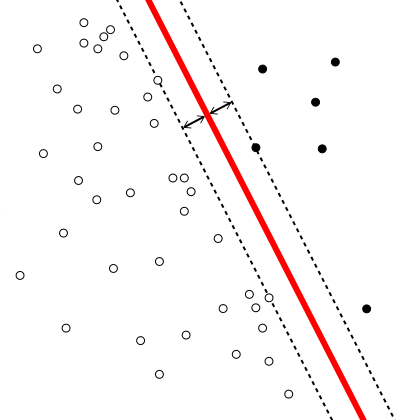
\includegraphics[width=0.41\textwidth]{img/Linear_Kernel_Machine.png}
		\caption{SVM: Linear Kernel}
		\label{f1}
	\end{minipage}
	\hspace{0.1cm}
	\begin{minipage}[t]{0.5\linewidth} 
		\centering
		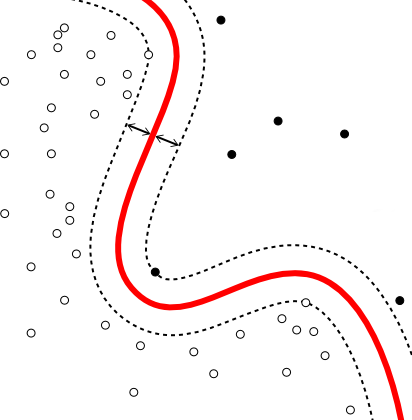
\includegraphics[width=0.41\textwidth]{img/Poly_Kernel_Machine.png}
		\caption{SVM: Polynomial Kernel}
		\label{f2}
	\end{minipage}        
\end{figure} 
\image{img/RBF_Kernel.png}{SVM: Radial Basis Function Kernel}{0.3}

Nonlinear SVM's operate in two stages:
\begin{itemize}
	\item Perform a non-linear mapping of the feature vector $x$ onto a high-dimensional space that is hidden from the inputs or the outputs.
	\item Construct an optimal separating hyperplane in the high-dimensional space.
\end{itemize}

\begin{equation*}
\begin{aligned}
&\text{max }\quad L_D(\lambda_1,\dots,\lambda_N) = \sum_{i = 1}^{N}\lambda_i - \frac{1}{2}\sum_{i = 1}^{N}\sum_{j = 1}^{N}\lambda_i\lambda_jy_iy_jx_i^Tx_j\\
&\text{s.t.} \quad \sum_{i = 1}^{N}\lambda_iy_i= 0 \qquad 0 \leq \lambda_i \leq C, \quad \forall i = 1,\dots,N\\
\end{aligned}
\end{equation*}
The discriminant function obtained from the solution is:
$$f(x) = \sum\limits_{i = 1}^Ny_i\lambda_ix_i^Tx +b$$
Suppose we first mapped the data to some other (possibly infinite dimensional) Euclidean space, using a mapping:
$$x \rightarrow \phi(x) \qquad K(x,y) = \phi(x)^T\phi(y)$$

\begin{equation*}
\begin{aligned}
&\text{max }\quad L_D(\lambda_1,\dots,\lambda_N) = \sum_{i = 1}^{N}\lambda_i - \frac{1}{2}\sum_{i = 1}^{N}\sum_{j = 1}^{N}\lambda_i\lambda_jy_iy_jK(x_i,x_j)\\
&\text{s.t.} \quad \sum_{i = 1}^{N}\lambda_iy_i= 0 \qquad 0 \leq \lambda_i \leq C, \quad \forall i = 1,\dots,N\\
\end{aligned}
\end{equation*}
$$f(x) = \sum\limits_{i = 1}^Ny_i\lambda_iK(x_i, x) +b$$
Note that is not necessary to compute $\phi(x)$.

\subsection{Multi-class problems}
Until now we have discussed about the application of an SVM just using two labels $y \in\{-1,1\}$. But in real case we can have more than two classes and we have to make an SVM which is able to assign input vector to one of the $K$ classes. In other words, we have to find a decision rule that divides the input space into $K$ decision regions separated by decision boundaries. 
\image{img/multiclass.png}{Space separation for 3 classes.}{0.3}
We can apply to distinct strategies:
\begin{itemize}
	\item \textbf{One-vs-the rest classifiers}, train $K-1$ classifiers each of which solves a two-class problem of separating points in a particular class from points not in that class.
	
	\item \textbf{One-vs-one classifiers}, train $k(k-1)/2$ binary classifiers, one for every possible pairs of classes.
	
\end{itemize}

\begin{figure}[!h]
	\begin{minipage}[t]{0.5\linewidth}
		\centering
		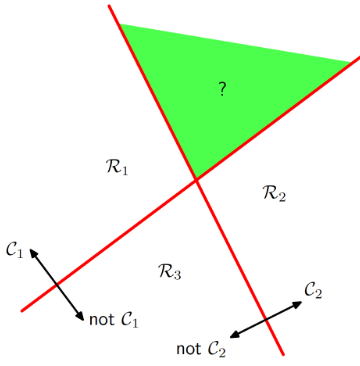
\includegraphics[width=0.51\textwidth]{img/onevsrest.png}
		\caption{One-vs-the-rest classifiers.}
	\end{minipage}
	\hspace{0.1cm}
	\begin{minipage}[t]{0.5\linewidth} 
		\centering
		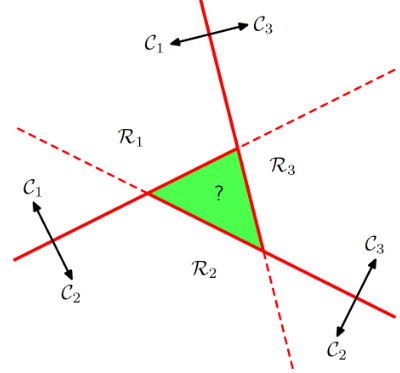
\includegraphics[width=0.51\textwidth]{img/onevsone.png}
		\caption{One-vs-one classifier.}
	\end{minipage}        
\end{figure} 
The classical approach consists on training $K$ one-vs-the rest classifiers and then the classification is done choosing the class with the most positive score.

\image{img/learnKclasses.png}{Decision boundaries on typical approaches.}{0.5}